
\section{Molecular Dynamics (MD) Simulations}

Molecular dynamics (MD) is a computational method used to analyze the interactions and movements of atoms and molecules. It offers better understanding of dynamic processes at atomic scale, such as diffusion, chemical reactions, and phase changes, making it an essential tool in physics, bioinformatics, molecular biology, materials science, and more. MD simulations are widely used to study protein folding, predict material properties, discover drugs, and analyze system behavior under various conditions \parencite{kukol2008molecular} \parencite{aktulga2012parallel}.
% [\textbf{existingTuning second reference, Downloads/978-1-59745-177-2.pdf}].

MD simulations begin with an initial configuration of particles, with specified positions and velocities. Forces acting on each particle are calculated using a force field, which defines the potential energy of the system. These forces are then translated into velocities and movements. Over discrete time steps, the positions and velocities of particles are updated, providing a dynamic view of the system's evolution.

% MD operates within the framework of classical mechanics, treating particles as point masses and neglecting quantum mechanical effects unless explicitly modeled using hybrid approaches. While this classical approach is suitable for many applications, phenomena such as chemical bond breaking or electronic transitions require reactive force fields or quantum mechanical methods [\textbf{existingTuning, parallelcomputing}].

\subsection{Computational Challenges and Optimizations}

While MD is a powerful tool, it is computationally expensive, requiring a significant amount of resources to deliver accurate and reliable results. The main challenges include handling large system sizes, modeling long simulation times, and more.

\subsubsection{Short-Range Simulations} \label{sec:shortrange}

To balance computational efficiency and accuracy of results, approximations are commonly introduced. While the distance between two particles increases, the pairwise forces between the two start converging to zero, and can therefore be ignored. For these types of potentials, called short-range potentials, a cutoff radius (\(r_c\)) is introduced. This approximation assumes that interactions beyond \(r_c\) are negligible and can be ignored. By doing so, the computational complexity is reduced from \(O(N^2)\) to \(O(N)\), where \(N\) is the number of particles. \parencite{gratl2022n}

% [\textbf{Gratl 2022.pdf}] 
% However, long-range potentials, while computable using advanced techniques, are not natively supported in AutoPas and are outside the scope of this discussion.

\subsubsection{Lennard-Jones Potential (LJ)}

The Lennard-Jones 12-6 potential is a widely used function in molecular dynamics simulations to model interactions between particles. It describes the balance between short-range repulsion and long-range attraction forces. This balance is given by:

\[
V(r) = 4\epsilon \left[ \left(\frac{\sigma}{r}\right)^{12} - \left(\frac{\sigma}{r}\right)^{6} \right],
\]

where \(r\) is the distance between two particles, \(\epsilon\) is the depth of the potential well, representing the strength of attraction, and \(\sigma\) is the distance at which the potential changes sign. \parencite{wang2020lennard}

The first term, \((\sigma/r)^{12}\), models the steep repulsive forces that dominate at very short distances, while the second term, \((\sigma/r)^{6}\), represents the weaker attractive van der Waals forces. The potential reaches its minimum value at \(r = 2^{1/6} \sigma\), which corresponds to the equilibrium distance between particles.

The Lennard-Jones potential is particularly suited for short-range interactions due to its rapid convergence to zero as \(r\) increases. \parencite{jones1924determination}

% [\textbf{jones1924determination, wang2020lennard, inproceedings for picture}].

\begin{figure}[ht]
\centering
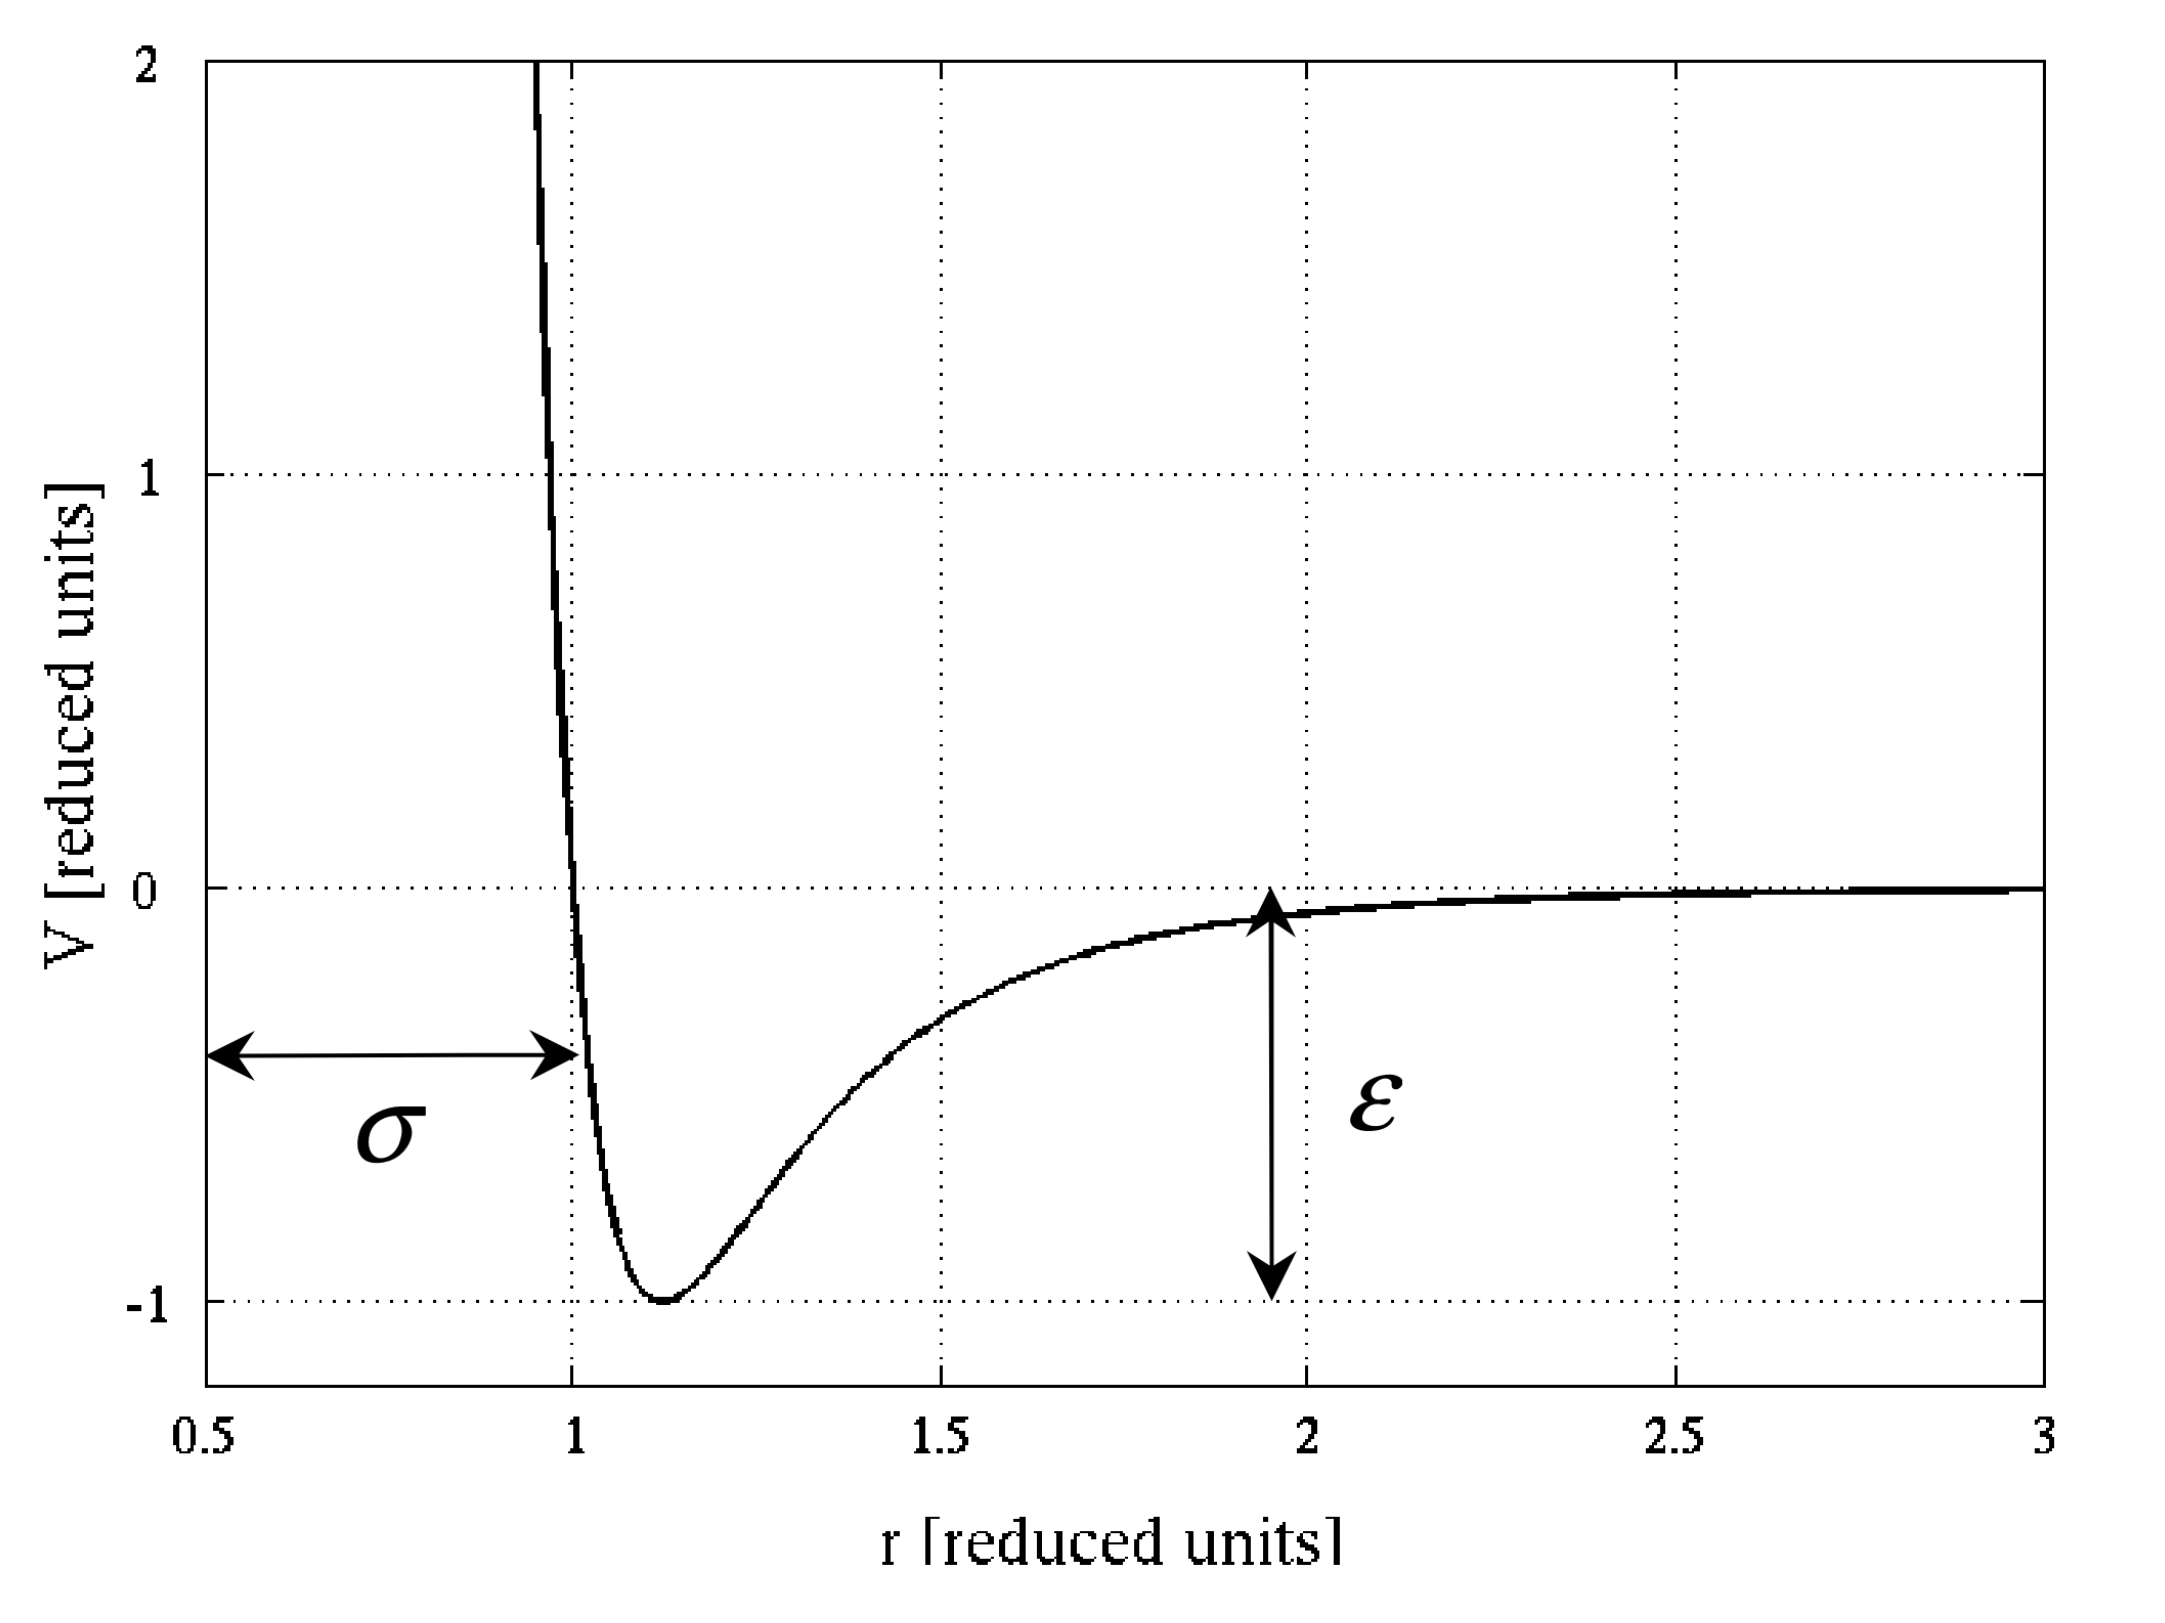
\includegraphics[%scale=1
                 width=0.5\linewidth, valign=t]{imgs/lj.png}
\caption{Lennard-Jones Potential \parencite{inproceedings}}
\label{lj}
\end{figure}



\subsubsection{Newton's Third Law}

An essential optimization in MD simulations is the application of Newton's third law, which states that every action has an equal and opposite reaction; or, the mutual actions of two bodies upon each other are always equal, and directed to contrary parts \parencite{frautschi1986mechanical}. 
In particle simulations, this means the force that particle \(p_1\) exerts on \(p_2\) is equal and opposite to the force \(p_2\) exerts on \(p_1\). Using this symmetry the number of force calculations is cut in half, significantly improving computational efficiency. In AutoPas, this optimization is implemented as the Newton3-optimization \parencite{gratl2022n}.
